\chapter{Multi-Party Computation}

\section{Introduction}
Multi-Party Computation (MPC), also known as Secure Function Evaluation, allows two or more parties
to correctly compute an agreed upon function of their private inputs without exposure, i.e., without
the input of one party being revealed to the other parties.\\
A generic function f receives as input a set $A = \{a_1,a_2,\dots,a_n\}$
of arguments and outputs a value z, as shown in Figure \ref{fig:mpcscheme}.\\
From that comes $z = f(a_1,a_2,\dots,a_n)$

\renewcommand{\figurename}{Figure}
\begin{figure}[H]
\centering
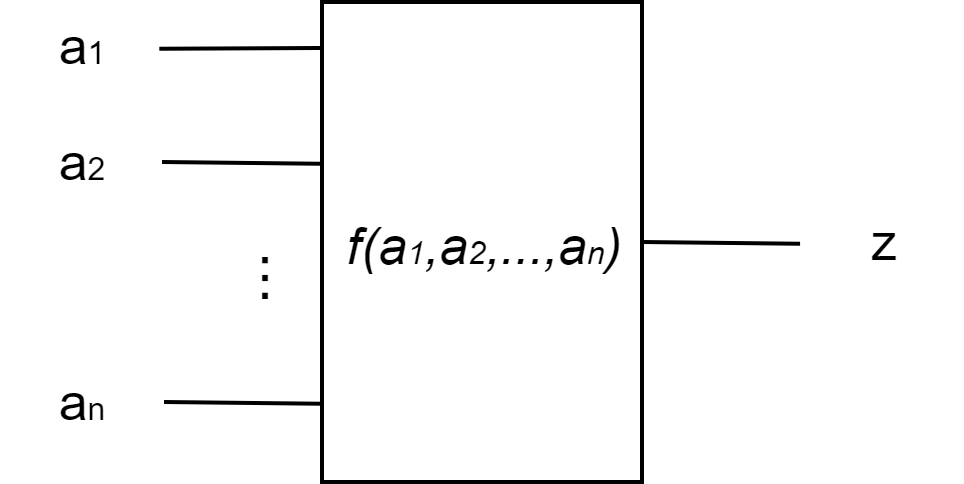
\includegraphics[width=.45\linewidth]{./figures/mpc_scheme}
\caption{Multi-Party Computation Scheme}
\label{fig:mpcscheme}
\end{figure}

\section{Two-Party Computation}
In 1986, Andrew Yao proposed the Garbled Circuit (GC) protocol, that addresses the specific case
of Two-Party Computation (2PC), without the presence of a trusted third party.\\
Two-Party Computation allows a secure evaluation of a function given
as a Boolean circuit that is represented as a series of logic gates.\\
For the case of 2PC, and much like MPC, a generic function f receives as input a set $A = \{a,b\}$
of arguments and outputs a value c, as shown in Figure \ref{fig:tpcscheme}.\\
From that comes $c = f(a,b)$

\renewcommand{\figurename}{Figure}
\begin{figure}[H]
\centering
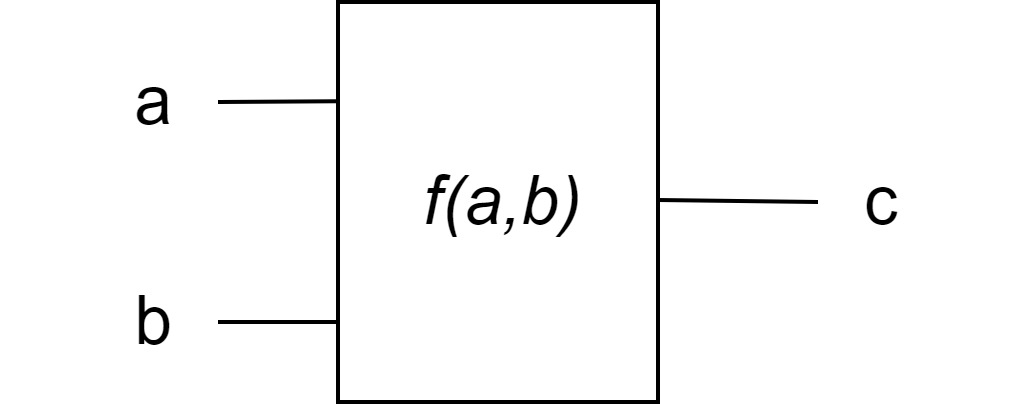
\includegraphics[width=.35\linewidth]{./figures/two_party_computation_scheme}
\caption{Two-Party Computation Scheme}
\label{fig:tpcscheme}
\end{figure}


\bibliography{./chapter/mpcomputation}